\section{Giới Thiệu}
\label{sec:intro}

Các mô hình ngôn ngữ lớn đa phương thức (Multimodal Large Language Models - MLLMs) chuyên biệt cho ảnh viễn thám (RS-MLLMs) như GeoChat \cite{geochat2024}, LLaVA-NeXT \cite{llavanext2024}, Qwen2.5/3-VL \cite{qwen2025vl} và InternVL \cite{internvl2025} đang dần trở thành giao diện phân tích thống nhất cho các tác vụ hỏi đáp trực quan (VQA), chú giải hiện trường và định vị đối tượng trên ảnh vệ tinh và viễn thám. Tuy nhiên, song song với năng lực lập luận mạnh mẽ, một thách thức dai dẳng và nguy hiểm được ghi nhận rộng rãi trong cộng đồng nghiên cứu là hiện tượng ảo giác (hallucination) khi đối tượng quan sát có kích thước nhỏ hoặc bị suy giảm độ phân giải \cite{radar2024, rshallu2024, uhrmicro2024}. Trong các ứng dụng nhạy cảm về an toàn như cứu nạn thiên tai, trinh sát quốc phòng hay quy hoạch đô thị, việc mô hình tự tin suy đoán sai lệch về sự hiện diện, chủng loại hoặc thuộc tính của đối tượng sẽ dẫn đến những quyết định sai lầm nghiêm trọng.

\begin{figure*}[t]
\centering
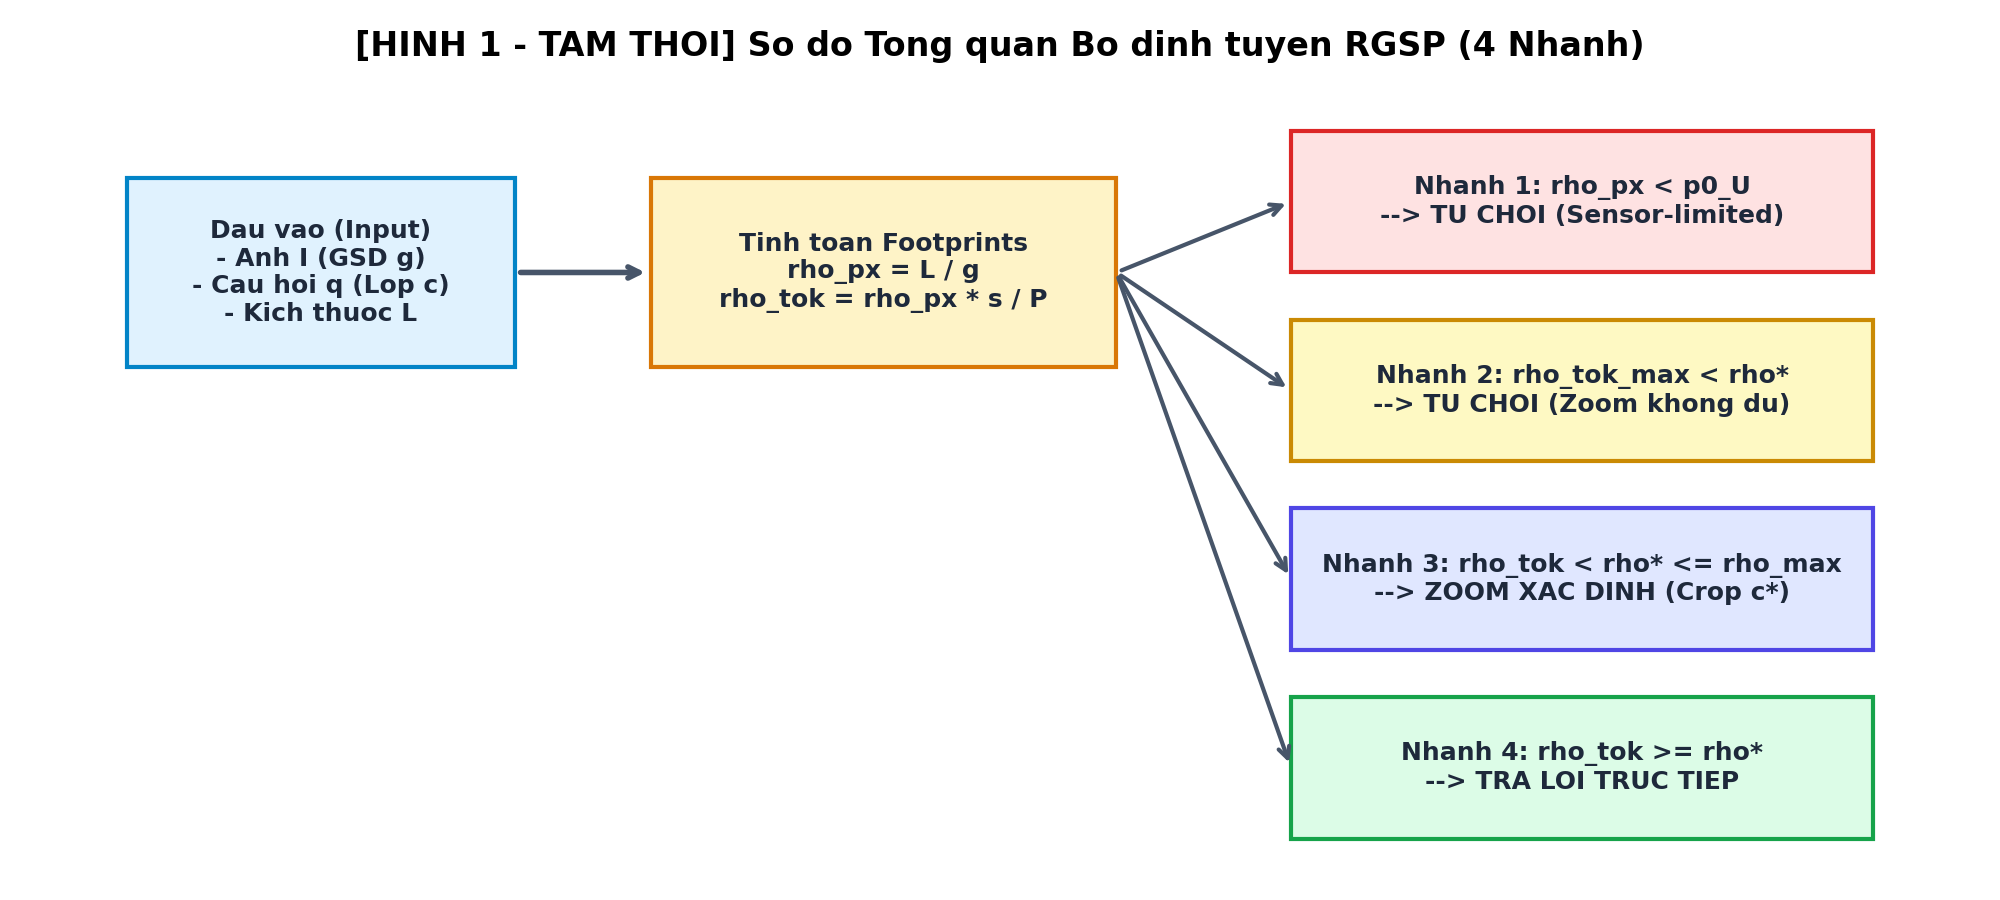
\includegraphics[width=0.92\textwidth]{figures/fig1_overview.png}
\caption{Tổng quan kiến trúc phương pháp RGSP: Phân tách hai nút thắt phân giải vật lý (Footprint pixel cảm biến $\rhopx$ và Footprint token bộ mã hóa $\rhotok$) và cơ chế định tuyến 4 nhánh không cần huấn luyện (Từ chối do cảm biến, Từ chối do trần token, Phóng đại thích nghi xác định và Trả lời trực tiếp).}
\label{fig:overview}
\end{figure*}

Các nghiên cứu gần đây đã bước đầu phân tách lỗi nhận thức của mô hình thành hai dạng: Type 1 (\textit{không tìm thấy}) do giới hạn tìm kiếm chú ý và Type 2 (\textit{không nhìn rõ}) do đối tượng quá nhỏ \cite{radar2024}, hoặc định nghĩa hiện tượng chênh lệch giữa độ phân giải vật lý và nhận thức trực quan là ảo ảnh độ phân giải (\textit{resolution illusion}) \cite{uhrmicro2024}. Mặc dù vậy, toàn bộ các nghiên cứu này đều tồn tại ba khoảng trống phương pháp luận then chốt:
\begin{enumerate}
    \item \textit{Chưa định lượng được giới hạn bằng biến số tính trước}: Các nghiên cứu trước chỉ phân tích thống kê sau khi mô hình đã trả lời sai, mà không có cơ chế toán học tính toán trước xác suất thất bại từ siêu dữ liệu cảm biến và kích thước vật lý của đối tượng.
    \item \textit{Chưa tách bạch hai nút thắt có hệ quả vận hành đối lập}: Thất bại có thể do vật thể không đủ thông tin trên ảnh gốc (giới hạn vật lý của cảm biến viễn thám) hoặc do vật thể có trên ảnh gốc nhưng bị nén triệt tiêu trong biểu diễn token (giới hạn kiến trúc của bộ mã hóa Vision Transformer).
    \item \textit{Thiếu cơ chế định tuyến xác định}: Các phương pháp đề xuất phóng đại (zoom) hiện nay \cite{radar2024, uhrmicro2024} đều áp dụng cắt ảnh thích nghi một cách mù quáng, gây lãng phí tài nguyên suy luận và thậm chí làm tăng ảo giác khi ảnh gốc vốn dĩ đã vượt quá giới hạn phân giải cảm biến.
\end{enumerate}

Vấn đề ``cần bao nhiêu điểm ảnh để nhận biết đối tượng'' đã được giải quyết thấu đáo trong quang học viễn thám truyền thống qua Tiêu chí Johnson (Johnson's Criteria, 1958) \cite{johnson1958analysis} và phương trình chất lượng ảnh tổng quát GIQE \cite{leachtenauer1997general}: số chu kỳ phân giải trên chiều tới hạn của vật thể quyết định khả năng phát hiện (\textit{detection}), định hướng (\textit{orientation}), nhận dạng (\textit{recognition}) và định danh (\textit{identification}). Tuy nhiên, khi đưa ảnh viễn thám vào MLLM, hệ thống xuất hiện đồng thời hai nút thắt thay vì một:
\begin{equation}
\rhopx = \frac{L}{\gsd}, \qquad \rhotok = \rhopx \cdot \frac{s_m(I)}{P_m},
\label{eq:footprints}
\end{equation}
trong đó $L$ là kích thước vật lý đặc trưng của đối tượng (mét), $\gsd$ là khoảng cách lấy mẫu mặt đất (Ground Sample Distance - GSD, mét/pixel), $s_m(I)$ là hệ số co giãn ảnh của mô hình $m$, và $P_m$ là kích thước patch hiệu dụng (pixel mô hình trên mỗi token) của bộ mã hóa ViT.

Đại lượng $\rhopx$ đo lường nút thắt cảm biến (đại lượng cổ điển của Johnson). Ngược lại, $\rhotok$ đo lường nút thắt bộ mã hóa - đại lượng hoàn toàn mới xuất hiện ở mạng nơ-ron đa phương thức. Nếu một chiếc xe có kích thước $L = 1.8\text{ m}$ chụp ở GSD $\gsd = 0.6\text{ m/px}$, nó chỉ chiếm đúng 3 pixel trên ảnh gốc; không có thuật toán phóng đại nào có thể tạo thêm thông tin thực tế từ 3 điểm ảnh này, và hành động duy nhất có trách nhiệm của hệ thống là từ chối trả lời (\textit{Abstain}). Nhưng nếu chiếc xe đó ở GSD $\gsd = 0.15\text{ m/px}$ (chiếm 12 pixel gốc) bị mô hình co về kích thước nhỏ và rơi lọt thỏm vào một patch 32 pixel của ViT, thông tin đã bị mất trong không gian token nhưng vẫn nguyên vẹn trên ảnh gốc; lúc này, phóng đại cục bộ (\textit{Zoom}) sẽ khôi phục lại khả năng giải quyết của mô hình.

Bài báo này giải quyết trọn vẹn bài toán trên thông qua việc trả lời ba câu hỏi nghiên cứu:
\begin{itemize}
    \item RQ1: \textit{Nút thắt token có thực sự tồn tại độc lập với nút thắt pixel trên các MLLM viễn thám hiện đại hay không?}
    \item RQ2: \textit{Làm thế nào để phân định một cách xác định trước suy luận: khi nào phóng đại có tác dụng, và khi nào bắt buộc phải từ chối?}
    \item RQ3: \textit{Tín hiệu vật lý tính trước ($\rhopx, \rhotok$) có kiểm soát rủi ro lựa chọn (selective risk) vượt trội hơn độ tin cậy logit nội tại của mô hình không?}
\end{itemize}

Đóng góp cốt lõi của bài báo gồm:
\begin{enumerate}
    \item Xây dựng bộ chuẩn RS-Resolve: Benchmark kiểm soát vật lý gồm 30.771 câu hỏi trắc nghiệm đa nhiệm vụ (Q1--Q6) được chuẩn hóa từ 5 tập ảnh vệ tinh lớn (DOTA-v2, DIOR, xView, VisDrone, iSAID), gắn nhãn đầy đủ $\rhopx, \rhotok$, GSD thực tế và cờ từ chối khách quan.
    \item Khảo sát và kiểm định thực nghiệm trên 5 RS-MLLM: Chứng minh bằng thực nghiệm trên 30.771 mẫu rằng hệ số hồi quy của nút thắt token $\beta_1 < 0$ có ý nghĩa thống kê áp đảo ($p < 10^{-11}$) trên tất cả các mô hình, xác nhận giả thuyết $H_1$.
    \item Đề xuất bộ định tuyến RGSP không cần huấn luyện: Thiết lập cơ chế định tuyến 4 nhánh (Từ chối cảm biến / Từ chối trần token / Phóng đại xác định / Trả lời trực tiếp) tích hợp kiểm soát rủi ro bằng \textit{fixed-sequence testing}, cho phép giảm mạnh ảo giác với chi phí tính toán bằng không trước suy luận.
\end{enumerate}
